\documentclass[tikz,border=10pt]{standalone}
\usetikzlibrary{calc}
\begin{document}
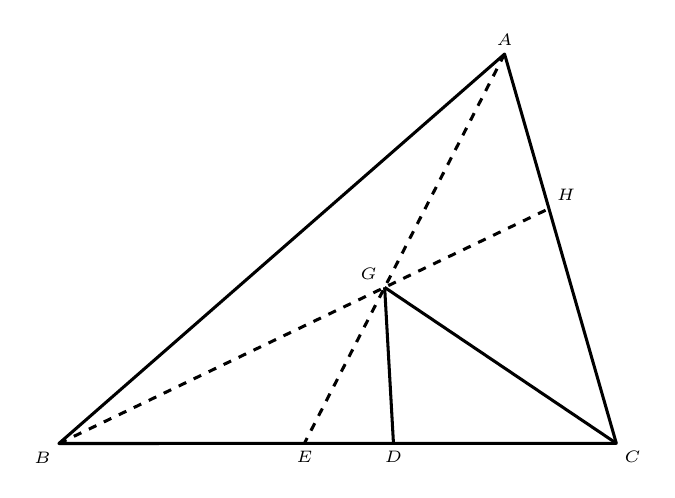
\begin{tikzpicture}[line width=1.1pt, line join=round]
% Coordinates from pixel measurements, s=0.009988, centred on ink bbox
\coordinate (B) at (-3.544,-2.478);
\coordinate (A) at (2.116,2.468);
\coordinate (C) at (3.535,-2.475);
\coordinate (E) at (-0.426,-2.476);
\coordinate (D) at (0.705,-2.476);
\coordinate (H) at (2.679,0.505);
\coordinate (G) at (0.593,-0.495);

% Solid triangle sides and inner solid segments
\draw (A) -- (B) -- (C) -- cycle;
\draw (G) -- (D);
\draw (G) -- (C);

% Dashed cevians through G
\draw[dashed] (A) -- (G) -- (E);
\draw[dashed] (B) -- (G) -- (H);

% Labels
\fontsize{6}{7.2}\selectfont
\node[below left] at (B) {$B$};
\node[below right] at (C) {$C$};
\node[below] at (D) {$D$};
\node[below] at (E) {$E$};
\node[above] at (A) {$A$};
\node[above right] at (H) {$H$};
\node[above left] at (G) {$G$};
\end{tikzpicture}
\end{document}